%%%%%%%%%%%%%%%%%%%%%%%%%%%%%%%%%%%%%%%%%
% Thin Sectioned Essay
% LaTeX Template
% Version 1.0 (3/8/13)
%
% This template has been downloaded from:
% http://www.LaTeXTemplates.com
%
% Original Author:
% Nicolas Diaz (nsdiaz@uc.cl) with extensive modifications by:
% Vel (vel@latextemplates.com)
%
% License:
% CC BY-NC-SA 3.0 (http://creativecommons.org/licenses/by-nc-sa/3.0/)
%
%%%%%%%%%%%%%%%%%%%%%%%%%%%%%%%%%%%%%%%%%

%----------------------------------------------------------------------------------------
% Packages and other document configurations
%----------------------------------------------------------------------------------------

\documentclass[11pt]{article} % Font size (can be 10pt, 11pt or 12pt) and paper size (remove a4paper for US letter paper)

\usepackage[protrusion=true,expansion=true]{microtype} % Better typography
\usepackage{graphicx} % Required for including pictures
\usepackage{wrapfig} % Allows in-line images

\usepackage{mathpazo} % Use the Palatino font
\usepackage[T1]{fontenc} % Required for accented characters
\linespread{1.275} % Change line spacing here, Palatino benefits from a slight increase by default

\usepackage[margin=1in]{geometry} % Reasonable margin size
\setlength{\parskip}{.3em}
\usepackage{amsmath}
\usepackage[hidelinks]{hyperref}
\usepackage{float}
\usepackage{booktabs}

\makeatletter
\renewcommand\@biblabel[1]{\textbf{#1.}} % Change the square brackets for each bibliography item from '[1]' to '1.'
\renewcommand{\@listI}{\itemsep=0pt} % Reduce the space between items in the itemize and enumerate environments and the bibliography

\renewcommand{\maketitle}{ % Customize the title - do not edit title and author name here, see the TITLE block below
\begin{flushright} % Right align
{\LARGE\@title} % Increase the font size of the title

\vspace{20pt} % Some vertical space between the title and author name

{\large\@author} % Author name
\\\@date % Date

\vspace{20pt} % Some vertical space between the author block and abstract
\end{flushright}
}

%----------------------------------------------------------------------------------------
% Title
%----------------------------------------------------------------------------------------

\title{\textbf{Musical Chairs:}\\ 
\vspace*{0.25em} % Title
Interpreting features that influence Billboard ranking} % Subtitle

\author{\textsc{Danny Vilela} % Author
\\{New York University}} % Institution

\date{\today} % Date

%----------------------------------------------------------------------------------------

\begin{document}

% Generate FERPA cover page
\topskip0pt
\vspace*{\fill}
\begin{center}
	Danny Vilela
\end{center}
\vspace*{\fill}

\newpage

%----------------------------------------------------------------------------------------

\maketitle % Print the title section

%----------------------------------------------------------------------------------------
% Essay body
%----------------------------------------------------------------------------------------

\section*{Introduction}

Practically gospel for up-and-coming and star-studded artists alike, the US Billboard is the \textit{de facto} source for determining a particular song's nationwide influence, and consistent top 5 placement is tantamount to cementing one's self as a musical icon. As a ranking for the nation's top 100 trending songs, the billboard has seen numerous iterations in its attempts to accommodate to ever-changing public outlets --- evolving from including only commercially-available songs to its modern, digital-platform (read: YouTube views, Spotify and Apple Music stream counts, AmazonMP3 and iTunes sales, etc.) inclusive equivalent. \par

In 2013, it was reported that the average iTunes user generates \$12 in music sales. This might not sound like much until you consider that iTunes alone accounted for roughly \$6.9 billion in annual consumer spending on music --- roughly three-fourths of global consumer spending for the 2012/2013 fiscal year. In the years since the music industry has seen a significant array of changes -- particularly in the meteoric rise of streaming services like Spotify and Apple Music. That said, it is evident that the Billboard top 100 accounts for much of this success: a higher profile on the billboard draws attention at the national level and often promotes artists to continue releasing music in hopes of capitalizing on said limelight. The opportunity to predict a particular song's success would have widespread utility: artists can better understand their standing within the musical industry, record labels can optimize their artists' position on the top 100, and both can optimize their release schedules to maintain a steady social reach. \par

\section*{Problem}
Given the unforgiving nature of the public's consumer interests paired with a short-term attention span, a series of poor rankings on the top 100 can quickly fade an artist's relevance and cause career-crippling effects. Artists who consistently fail to break the top 100 are seldom considered ``successful'' by record companies, investors, and -- most importantly -- the public. \par 

As a result, we are interested in examining what readily-available factors can be determined to be most influential towards any particular song's ranking within the top 100. Naturally, we approach our prediction problem: how can we best predict a song's success? This problem has numerous dimensions that our dataset will not be able to account for -- including the artist's ``image'' and practically everything not explicitly influencing billboard ranking -- and so we approach this task by limiting ourselves to publicly-available, quantified billboard ranking data. We seek to determine if we can model a song's peak chart placement through historical data, and if so, what particular predictors can best perform said task. \par

Given we are concerned with a song's peak overall chart position, we are tasked with determining which predictors will give us our best estimate. We rationalize that a mixture of a song's inherent features will allow us to best determine its peak chart position. Naturally, we include the provided predictors:
\begin{enumerate}
	\item our song's position last week: \texttt{last\_week\_position}
	\item our song's current peak position: \texttt{current\_peak}
	\item how long our song has been on the current top 100 chart: \texttt{weeks\_on\_chart}
	\item our song's entry position into the top 100: \texttt{entry\_position}
	
\end{enumerate}

and our calculated predictor:
\begin{enumerate}
	\item our artist's ``relevance score'' for the decade in question: \texttt{artist\_relevance}
\end{enumerate}

%Note: \texttt{concurrent\_count} is determined by the number of songs our artist concurrently has in the top 100 \textit{for that particular chart date}. For example, if Rihanna has 3 songs on the 6 September 2014 billboard, her \texttt{concurrent\_count} rating is 3 for all 3 of her billboard top 100 songs. If in the following week she releases another song that debuts onto the top 100, each of her songs will have a \texttt{concurrent\_count} rating of 4 on that chart table, and so on. It seems evident, but I predict that if an artist has a higher concurrent count, we can expect that their next release is more likely to enter the top 100. \par

\texttt{artist\_relevance} is calculated by noting how many unique songs an artist has released in our dataset's time frame. So, for example, Rihanna will have a \texttt{artist\_relevance} score of 29 if, from 2010 to 2016, 29 of her songs have entered the top 100 on the billboard chart. Again, it seems almost obvious, but I predict that if an artist has a higher relevance score, their next song is more likely to enter the top 100. \par

\section*{Regression Model}

\subsection*{Model Definition}
We can represent our earlier assertion through the linear regression model:
\[ \text{Peak chart position} =  \beta_0 + \beta_1 \times \texttt{last\_week\_position} + \beta_2 \times \texttt{current\_peak} \] 
\[\hspace*{10.1em} + \beta_3 \times \texttt{weeks\_on\_chart} + \beta_4 \times \texttt{entry\_position} \]
\[\hspace*{0.5em} + \beta_5 \times \texttt{artist\_relevance} \]

We note that a song that has yet to be released will have profound impacts on our ability to predict its overall peak chart position. Furthermore, our model seems incomplete in that it seems to apply a slightly-too-harsh of a penalty for artists who have never released a song in a particular decade, since all predictors will be 0. That said, the limits of our dataset do not allow us to speculate about an artist's appeal or ability to meet consumer demand, and so we have few alternative choices.

\subsection*{Regression Validation}
Before approaching a dataset with the mindset of performing a linear regression, it was necessary to validate that the conditions for performing a regression analysis of our data was an appropriate route.

\begin{enumerate}
	\item \textbf{$E(\epsilon_i) = 0\ \forall\ i$}: No members of the population -- that is, songs released by artists -- are systematically above or below the regression line due to the nature of the billboard's ranking: if a song is popular among fans, is played often on the radio or other music media (MTV, Spotify, Apple Music), and is selling well through physical and digital mediums (iTunes, AmazonMP3), it will be ranked accordingly. We rely upon the billboard's algorithm for determining song ranking to be robust in that it does not inherently prefer certain songs by certain artists (this is different from a well-known artist's song doing well -- leveraging virality/popularity $\neq$ inherent bias).
	
	\item \textbf{$V(\epsilon_i) = 0\ \forall\ i$}: We note that the homoscedasticity within this dataset is referring to the equal playing field for all songs to possibly achieve a peak ranking of 1. It is \textbf{not} the case that relationship between the predictors and our response variable is more inherently tied for certain songs. As previously stated, all songs are given the same opportunity to rank highly on the chart -- there is no assumed inherent bias on behalf of the billboard ranking algorithm -- and so we assert that the $x$/$y$ relationship is \textbf{not} stronger for some members of the population and weaker for others.
	
	\item $\epsilon_i$ and $\epsilon_j$ are not correlated with each other for $i \neq j$: This is fundamentally assured due to the randomness of our dataset: it would be impossible to assert that knowing observation $i$'s expected value will tell us anything about observation $j$'s (or $k$'s, $m$'s, etc.) expected value. The only such case where knowing observation $i$'s expected value would be able to tell us anything about observation $j$'s expected value would be if the same artist for song $i$ released a song $j$ with the exact same ``environment'' -- that is, media attention, public interest, etc -- which cannot be true for any observations $i$ and $j$. No expected values within our dataset are correlated because it would not be possible for a song $i$ to also be a song $j$ on the \textbf{same chart}. Anywhere that a value could be double-counting (such as when calculating \texttt{artist\_relevance}) -- and thus where a value $\epsilon_i$ could be correlated with $\epsilon_j$, I took extreme precaution to only observe the observation $i$ in a time frame where it is the only instance of $i$. Therefore, there cannot be a correlation between expected values when $i \neq j$.
	
	\item $\epsilon_i \sim N(0,\ \sigma^2)$: Given that our data contains a large number of observations with peak rankings ranging across the spectrum, we can assume our data represents a normal distribution.
\end{enumerate}

Because we can show that these assumptions hold, we know that least squares regression is the proper regression to use. \par

\section*{Data Sourcing, Cleaning, Engineering}
I sourced my data by using GitHub user \href{https://github.com/guoguo12/billboard-charts}{\texttt{guoguo12}'s \texttt{billboard-charts}} parser, which utilizes a Python interface in order to query   and scrape data from Billboard's \href{http://www.billboard.com/charts/hot-100}{\texttt{website}} and generate a pipe-separated text file with numerous features for each song in the top 100. Afterwords, I utilized \textsc{R} in order to parse, clean, and prepare the data for analysis. During said analysis, I wrote code in order to produce variables of my own that I felt would be relevant to our regression model's design. \par

The data's original form contained every weekly top 100 entry stretching from its debut in 1940 to March 2015. This particular analysis will use a subset of that data -- the top 100 charts from 2010 and onward -- as its main focus. We note that a model that is well-performing on the top 100 charts of 2010 and onward may not perform as well on top 100 charts from 2000 to 2010 or even 1990 to 2000 due to fundamental external changes in the top 100's ranking algorithm and advancements in music consumption. \par

Stripping our data down from all top 100 entries since 1940 to just the top 100 entries from 2010 and onward reduces our data by just over 90\% -- from 343 thousand to 27 thousand observations. We note that our data is misleading: the top 100 charts did \textbf{not} contain 27 thousand different songs over 6 years -- rather, there have been 100 entries every week for approximately 270 weeks, resulting in 270 thousand rows. Hence, our data contains many duplicates to be accounted for across different top 100 dates. \par

\subsection*{Data Validation}
Upon obtaining the data, I noticed that songs that were just debuting onto the top 100 had ``NEW'' in their \textbf{last.week} column, which proved problematic when determining the impact of our first predictor, \texttt{last\_week\_position}. To account for this, I set any song who had yet to debut onto the top 100 (and as such, had ``NEW'' in that field) to rank 101 in order to standardize what it meant to be new on the top 100. \par

A more fundamental dataset design problem that I had to keep in mind was that there would be an \textbf{enormous} amount of repetitive data. Given that this is tracking song position over time, I knew that a particular song could be seen multiple times in a particular timeframe of chart updates. \par

\subsection*{Predictor Engineering}
In order to determine the values for our additional, calculated predictor I had to consider how calculating these values would impact their representation. It was important to constantly keep the inherent overlapping of data in mind in order to prevent redundant, erroneous values. A brief explanation of the methodology for the calculated value is as follows:\par

\begin{enumerate}
	\item In order to generate values for \texttt{relevance score}, it was necessary first to \textit{split} our original \texttt{after\_2010} dataset such that we were interfacing with each individual chart entry from Jan 2010 to March 2015 (in other words, splitting one dataset into 271 100-line tables). Next, for each chart entry $c_{i}$ we identify all unique artists within a chart, identify each unique song by a unique artist within our time frame dataset, and write that value into $c_{i}$'s \texttt{relevance\_score} field.
\end{enumerate}

\section*{Exploratory Data Analysis}
First, let's take a quick look at a summary of our provided data:

\begin{verbatim}
 > summary(after_2010)

       pos          last.week          peak       weeks.on.chart
 Min.   :  1.00 | NEW    : 2703 | Min.   :  1.00 | Min.   : 1.0  |
 1st Qu.: 25.75 | 1      :  271 | 1st Qu.: 12.00 | 1st Qu.: 4.0  |
 Median : 50.50 | 10     :  271 | Median : 37.00 | Median :10.0  |
 Mean   : 50.50 | 15     :  271 | Mean   : 40.37 | Mean   :11.7  |
 3rd Qu.: 75.25 | 19     :  271 | 3rd Qu.: 65.00 | 3rd Qu.:17.0  |
 Max.   :100.00 | 2      :  271 | Max.   :100.00 | Max.   :85.0  |
                | (Other):23042 |                                
                  
          title                    artist             chart.entry.date     
 Radioactive        :   92 | TAYLOR SWIFT   :  387  |  Min.   :39865   |
 Sail               :   79 | BRUNO MARS     :  274  |  1st Qu.:40586   |
 Counting Stars     :   68 | KATY PERRY     :  263  |  Median :41041   |
 Party Rock Anthem  :   68 | LADY ANTEBELLUM:  261  |  Mean   :41050   |
 Rolling In The Deep:   67 | LUKE BRYAN     :  249  |  3rd Qu.:41517   |
 Ho Hey             :   62 | IMAGINE DRAGONS:  235  |  Max.   :42070   |
 (Other)            :26664 |  (Other)        :25431 |        
                            
 entry.position      overall.peak      overall.weeks.on.chart       chart.date      
  Min.   :  1.00 | Min.   :  1.00   |     Min.   : 1.00       |  Min.   :20100102  |  
  1st Qu.: 60.00 | 1st Qu.:  8.00   |     1st Qu.:16.00       |  1st Qu.:20110416  |
  Median : 88.00 | Median : 27.00   |     Median :20.00       |  Median :20120804  |
  Mean   : 73.84 | Mean   : 31.93   |     Mean   :21.98       |  Mean   :20121720  |
  3rd Qu.: 95.00 | 3rd Qu.: 51.00   |     3rd Qu.:26.00       |  3rd Qu.:20131123  |
  Max.   :100.00 | Max.   :100.00   |     Max.   :85.00       |  Max.   :20150307  |
\end{verbatim}

This summary data tells us a lot about our dataset and how we should be approaching our analysis. In particular, certain fields are strongly meaningless and deriving summary statistics provide little to no benefit towards understanding the analysis at hand. Some summary examples include:

\begin{enumerate}
	\item Our position tracker \textbf{pos}, chart date \textbf{chart.date}, and chart entry date \textbf{chart.entry date} tell us nothing about our data on their own. Given 271 top 100 charts, it must be true that the smallest and largest possible positions are 1 and 100, respectively. Chart date and chart entry date are meaningless without context.
	\item Our prior-week tracker \textbf{last.week} gives us some insight: it seems as though it is 10 times more likely that a song breaks into the top 100 from sub-100 ranking than it is for a song to internally go from top 100 to top 100 ranking.
	\item The median and mean \textbf{peak} descriptors tell us that an particular song on the top 100 will more or less gravitate towards rank 38.
	\item Our \textbf{title} field says little about the data, but it seems to contradict our previous point about ``Radioactive'' staying on the charts for 85 weeks. In fact, the discrepancy can be traced back to Kings of Leon releasing a song by the same name in 2010 (whereas the more popular ``Radioactive'' was released in 2012).
	\item Our \textbf{artist} field tells us the total number of times we've seen a particular artist over the six-year period. We can see (with little surprise) that pop-icons Taylor Swift, Bruno Mars, and Katy Perry lead the charts for overall relevance. Note that this frequency is different from the calculated \texttt{relevance\_score} statistic, since ``Drake'' \textbf{will not} be accounted for in this summary statistic if the artist is ``Rihanna ** Drake'', where ``**'' is any of ``feat.'', ``featuring'', ``and'', ``,'', or any other separator. \texttt{relevance\_score} accounts for this and instead does an entire substring search over the \textbf{artist} string field.
	\item Another interesting statistic is \textbf{entry.position}, which tells us the position at which any particular song entered the top 100. Our data is incredibly left-skewed, with most of our songs entering the top 100 in the bottom 40 ranks. That said, we note that some songs have actually \textit{debuted} at number 1 on the top 100, presumably incredibly difficult. After further investigation, these songs proved to be incredibly -- almost explosively -- viral, including Taylor Swift's ``Shake it Off'' and Baauer's ``Harlem Shake''.
	\item The total overall week tracker \textbf{weeks.on.chart} gives us very interesting insights into a song's staying power. Most songs are able to maintain approximately 10 weeks within the top 100 before falling out of favor, however we note a particularly interesting song who was able to stay in the top 100 for an astounding 85 weeks. This song -- ``Radioactive'' by IMAGINE DRAGONS -- was a viral hit, used in movie soundtracks, commercials, and many, many more. Exploring the data further, it was interesting to see that the song's last week in the top 100 had the song plummit from rank 49 to sub-100.
\end{enumerate}

Now, let's plot the relationship between a song's overall peak and the number of weeks it has been on the charts:

\begin{figure}[H]
	\label{Figure 1}
	\caption{Scatterplot of a song's particular song's relationship between number of weeks on chart and its ongoing peak}
	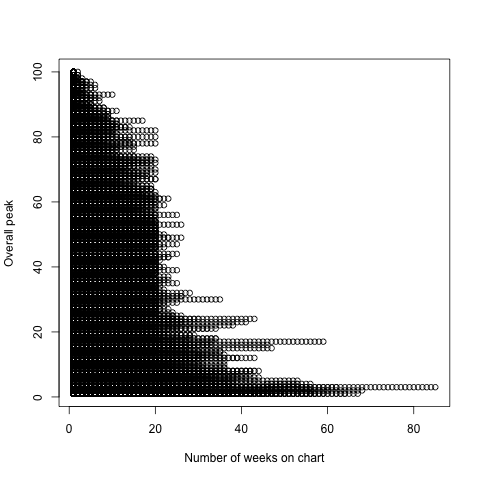
\includegraphics[scale = 0.5]{plots/weeks_v_overall_peak}
	\centering
\end{figure}

This data seems to be a noisy set of data points -- but we can glean a few interesting insights from what's there. In particular, we note that most songs do not last more than approximately 20 weeks on the chart, and that longer-lasting songs tend to champion the hot 100 given their breakout velocity. Given that songs at the very top left of the graph have short staying power and -- perhaps subsequently -- a lower rank on the chart, we can find some evidence that would support an inversal relationship between number of weeks on chart and overall peak --- that is, a larger staying power might result in a peak closer and closer to the top.

For reference, let's view the scatterplots of \textbf{overall.peak} in relation to all other predictors:

\begin{figure}[H]
	\label{Figure 2}
	\caption{Scatterplot of all pairs between our predictors}
	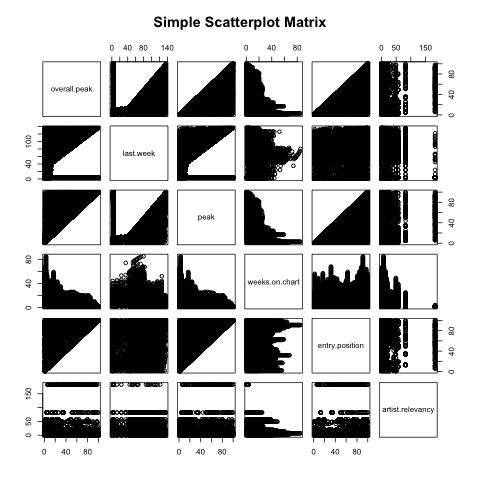
\includegraphics[scale = 0.5]{plots/pairs}
	\centering
\end{figure}

We note that there is no need to modify any of our predictors through logarithmic or power transformations -- their raw values will suffice. Let's also look at our predictor variables' correlations:

\begin{verbatim}
> cor(
+   cbind(after_2010$overall.peak, 
+      after_2010$last.week, after_2010$peak, after_2010$weeks.on.chart,
+      after_2010$entry.position, after_2010$artist.relevance
+   )
+ )

Correlations
                  over.p    last.wk   peak     wks.on.chrt entry.pos art.rele
overall.peak      1.000000
last.week         0.221202  1.000000   
peak              0.846744  0.240058  1.000000
weeks.on.chart   -0.457873 -0.039673 -0.606853  1.000000
entry.position    0.433522  0.198551  0.502938 -0.062878   1.000000
artist.relevance -0.000920 -0.133534 -0.032095 -0.085049  -0.121226  1.000000
\end{verbatim}

We note a few interesting things. Primarily, we see ones along the diagonal and soon realize that, of course, a coefficient \textit{must} be correlated to \textit{itself}. We also see a mixed amount of multicollinearity across our predictor variables, implying that an increase in one predictor results in a decrease in another. In particular, we see that some of our predictors have negative correlation values. Because our regression uses around half of our available features and two features based on other internal features, we may have several redundant variables whose impact on our regression is minimal, at best. Let's look at our regression output:

\begin{verbatim}
------------------------------------------------------------------------------
> summary(prediction_a)

Residuals:
	  +---------+--------+---------+--------+--------+
	  |   Min   |   1Q   | Median  |   3Q   |  Max   |
	  +---------+--------+---------+--------+--------+
	  | -73.721 | -3.548 |  1.678  |  7.527 | 27.087 |
	  +---------+--------+---------+--------+--------+ 

Coefficients:
                   +-----------+------------+---------+----------------+
                   | Estimate  | Std. Error | t value |    Pr(>|t|)    |
+------------------+-----------+------------+---------+----------------+
| (Intercept)      | -2.661721 |  0.878826  |  -3.029 |   0.00246  **  |
| last.week        |  0.521330 |  1.305651  |   0.399 |   0.68968      |
| peak             |  0.813077 |  0.007585  | 107.197 | < 2e-16    *** |
| weeks.on.chart   |  0.271192 |  0.012188  |  22.251 | < 2e-16    *** |
| entry.position   | -0.019872 |  0.003880  |  -5.121 |   3.06e-07 *** |
| artist.relevance |  0.052795 |  0.004673  |  11.297 | < 2e-16    *** |
+------------------+-----------+------------+---------+----------------+

---
Signif. codes:  0 `***' 0.001 `**' 0.01 `*' 0.05 `.' 0.1 ` ' 1
---

Residual standard error: 13.94 on 26995 degrees of freedom
Multiple R-squared: 0.7252,    Adjusted R-squared: 0.7242
F-statistic: 685.1 on 104 and 26995 DF,  p-value: < 2.2e-16
------------------------------------------------------------------------------
> vif(prediction_a)

VIF:
                   +----------+-----+-----------------+
                   |   GVIF   | Df  | GVIF^(1/(2*Df)) |
+------------------+----------+-----+-----------------+
| last.week        | 5.403777 | 100 |     1.008471    |
| peak             | 7.281167 |   1 |     2.698364    |
| weeks.on.chart   | 1.965529 |   1 |     1.401973    |
| entry.position   | 1.698464 |   1 |     1.303251    |
| artist.relevance | 1.061266 |   1 |     1.030178    |
+------------------+----------+-----+-----------------+

Regression Equation

Overall peak = -2.661721 + 0.521330 last week position + 0.813077 current peak
                         + 0.271192 weeks on chart - 0.019872 entry position
                         + 0.052785 artist relevance
\end{verbatim}

The regression fit, unfortunately, is not incredibly strong. One aspect of our data to keep in mind is that when we refer to a one unit increase in last week's position, we are referring to going \textbf{down} the rank by one position (e.g.: last week's position was 30. This week's position is 31. Ergo, we have gone \textbf{down} the chart --- closer to falling off). The coefficients can be interpreted as follows:
\begin{enumerate}
	\item A one unit increase in \textbf{last week's position} is associated with a 0.521 position increase on the billboard, bringing us closer to being bumped out of the top 100, holding all else fixed.
	\item A one unit increase in our \textbf{ongoing peak} (again, bringing us closer to being out of the top 100) is associated with a 0.813 position increase towards the bottom of the billboard, holding all else fixed.
	\item A one unit increase in the \textbf{number of weeks our song has been on the chart} has a slight decay factor -- all else held fixed, that increase is associated with a drop on the ranking by 0.2712 position.
	\item A one unit increase in our \textbf{entry position} is associated with a rise in the billboard chart by 0.0199 places, all others held fixed.
	\item A one unit increase in the \textbf{artist relevance} -- that is, how many songs an artist has released in a particular time frame -- is associated with a fall in the billboard ranking of 0.0528.
\end{enumerate}

We note the moderate amount of redundant variables -- seen where a predictor variable's $t$-statistic proving insignificant. We further note relatively low variance inflation factors across the board, given that a good guideline for VIF for this particular regression would be:
\[ VIF < max(10, \frac{1}{1 - R^{2}_{model}}) \rightarrow VIF < max(10, \frac{1}{1 - 0.7252}) \rightarrow VIF < max(10, 3.639)\]

That said, we also note the relatively low $R^{2}$ as a potential point of concern. Despite our predictors, our model only explains 72\% of the variability of the response data around its mean. 

\subsection*{Model Selection}
Given our proposed regression model, we further our analysis by considering how to determine if we can simplify our model such that we can perhaps balance fit on the regression and predictor simplicity -- and if so, what ``best'' model or set of ``best'' models will serve us best. Using a best subsets regression, we can consider the effects of limiting our model to 1, 2, ..., p predictors and better understand the pivotal predictors that truly make our model. Here is the output:

\begin{verbatim}
> leaps(
+   cbind(
+     after_2010$last.week, after_2010$peak, after_2010$weeks.on.chart, 
+     after_2010$entry.position, after_2010$artist.relevance), 
+     after_2010$overall.peak, 
+     nbest = 2
+ )

Note: 
   last.week        -> [1]
   peak             -> [2]
   weeks.on.chart   -> [3]
   entry.position   -> [4]
   artist.relevance -> [5]
   
Vars    R^2     R^2 (adj)   Mallows_Cp       S   [1]   [2]   [3]   [4]   [5]
  1  71.69767   71.69663     648.16211   14.12          X
  1  20.96479   20.96187   50380.51195    23.6                X
  2  72.19368   72.19163     163.93464      14          X     X
  2  71.76668   71.76460     582.51190    14.1          X                 X
  3  72.32219   72.31913      39.95772   13.96          X     X           X
  3  72.22284   72.21977     137.34667   13.99          X     X     X
  4  72.34240   72.33832      22.14496   13.96          X     X     X     X
  4  72.33920   72.33512      25.28558   13.95    X     X     X           X
  5  72.36091   72.35581       6.00000   13.94    X     X     X     X     X
\end{verbatim}

Since we are interested not only in how each predictor influences our overall peak chart ranking but also \textit{which} predictors do so the best, we do not express any mandates for our subset algorithm to include any particular predictor. 

To choose our best model(s) we first go down the list, observing each subset models' $R^{2}$ value and at what $p$ does it begin to plateau. We note that our $R^{2}$ begins to level-off at approximately \\ \textbf{p = 3}. We then look to maximize our adjusted $R^{2}$, and find that our models' $R^{2}_{a}$ begins to taper off at \textbf{p = 3 or p = 4}. Next, we look to utilize a model whose $C_{p}$ criterion best satisfies $C_{p} \leq p + 1$ and/or minimize($C_{p}$). We note that when \textbf{p = 5}, both the minimum $C_{p}$ is found and $C_{p} \leq p + 1$ is closest to an exact fit. Lastly, we look to Akaike's information criterion and criterion corrected to determine our model selection. Let's look at our $AIC$ and $AIC_{c}$ values:

\begin{verbatim}
Vars          AIC                  AIC_c
   1  -177761.78259715307    -177761.78171141347
   1  -163841.7461900618     -163841.7453043222
   2  -177991.07845354368    -177991.07697725654
   2  -177798.19507700743    -177798.1936007203
   3  -178066.61784835963    -178066.6156338472
   3  -178008.4425129599     -178008.44029844747
   4  -178064.61784835963    -178064.6147479278
   4  -178084.0374120713     -178084.03431163947
   5  -178101.47090160972    -178101.466767548
\end{verbatim}

We note that our minimum $AIC$ is seen when \textbf{p = 1}, and that our minimum $AIC_{c}$ value is also seen when \textbf{p = 1}.

We unfortunately note that our available criterion do not seem to be approaching or suggesting any particular p. While our first two tests advocate for a p = 3 or p = 4, both p = 3 and p = 4 are far from being contenders for our fourth criterion where we attempt to reduce $C_{p}$. Our final two criterion seem to vote for a model where p = 1, which tells us that there doesn't seem to be any particularly-agreeable subset of predictors among our five that can serve as a simpler model for our regression.

\section*{Summary}
Despite our best efforts, there does not seem to be a strong case in support of the notion that our 5 predictors can confidently predict a song's overall peak ranking on the billboard top 100. One potential explanation for this is, as previously mentioned, new artists who are making their debut into the top 100 are harshly penalized and their rank is weighed down considerably. Furthermore, it could be that the data aggregated by the billboard top 100 just isn't a sufficient or thorough representation of how the public ranks artists. Given that popular musicians are not just musicians and celebrities but social media icons, actors, and more, it is more likely that there are greater forces at work that impact a particular artist's song's ranking.

I had intended on including another calculated predictor, \texttt{concurrent\_count}, which would tell us the number of songs a particular artist that were already within the top 100 for any particular chart spanning the time frame. Unfortunately, RStudio crashed and it would have meant this submission being late if I had decided to re-run the calculations (for reference, the calculation for just the post-2012 charts had already taken 6.5 hours). After submitting this report, I will try calculating this predictor and personally noting if \texttt{concurrent\_count} significantly contributes to our regression fit.

This analysis proved considerably more difficult than my previous analysis. In particular, attempting to calculatie \texttt{concurrent\_count} required quite a bit of trial and error, and despite optimizing my code for performance, just computing those two predictors for the partially-incomplete decade/dataset \texttt{after\_2010} took hours to run.

That said, I gained a much better understanding of R's internal data structure utilization and programming schema/syntax. Unlike my previous analysis, this report's prototyping/data exploration phase was more about understanding the underlying trends within the data and not as hindered by my unfamiliarity with R as a tool for data analysis. Ultimately, I learned more about statistical reporting and, in particular, the data modeling process -- that is, going from question $\rightarrow$ data $\rightarrow$ model $\rightarrow$ validation $\rightarrow$ analysis $\rightarrow$ results.

In retrospect, had our regression been more useful and described our data more wholly, it would have been ideal to cross-validate our regression model on other decades of our billboard data.

%----------------------------------------------------------------------------------------
% Resources
%----------------------------------------------------------------------------------------
\subsection*{Resources}
All files pertaining to this statistical report, including the \texttt{R} data analysis script, dataset, plots, and this PDF report are open to the public and hosted on GitHub (\href{https://github.com/dannyfig/MultivaRiate/tree/master/Multiple_Linear_Regression}{\url{github.com/dannyfig/multivariate/multiple_linear_regression}}).

%----------------------------------------------------------------------------------------
% Data
%----------------------------------------------------------------------------------------

\subsection*{Data}
Below is a slice (\textbf{pivoted in order to fit}) of the billboard dataset I utilized for this statistical analysis report. A few points to note are as follow:
\begin{enumerate}
	\item Originally, the parsed dataset provided 10 relevant features. Notably: \textbf{last week} (song's position last week, if applicable), \textbf{peak} (song's current billboard peak), \textbf{weeks on chart}, \textbf{title}, \textbf{artist}, \textbf{chart entry date}, \textbf{entry position}, \textbf{song's overall peak}, \textbf{overall weeks on chart}, \textbf{chart date} (date that data was recorded in YYYYMMDD format).
	\item Through some engineering within my \texttt{regression\_analysis.R} script, I was able to add an extra column, \textbf{relevance\_score}, which represented how many unique songs that artist had released in a set time frame (default: per decade).
\end{enumerate}

\begin{table}[H]
	\centering
	\begin{tabular}{|l|c|c|}
		COLUMNS & row\_1 & row\_2 \\
		last week              & 1 & 2 \\
		peak                   & 1 & 2 \\
		weeks on chart         & 15 & 20 \\
		title                  & ``Uptown Funk!'' & ``Thinking out loud'' \\
		artist                 & ``MARK RONSON featuring BRUNO MARS'' & ``ED SHEERAN'' \\
		chart entry date       & 41972 & 41937 \\
		entry position         & 65 & 69 \\
		overall peak           & 1 & 2 \\
		overall weeks on chart & 15 & 20 \\
		chart date             & 20150307 & 20150307 \\
		artist relevance       & 1 & 11
	\end{tabular}
\end{table}

%----------------------------------------------------------------------------------------

\end{document}